\documentclass[10pt,presentation,compress]{beamer}

\usepackage{graphicx}
\usepackage{parskip,amssymb,amsmath,amsthm,url}
\usepackage{subfigure}
\usepackage{esdiff}
\usepackage{latexsym}
\usepackage{color}

\title{How to choose a good colour map}
\author{Damon McDougall}
\institute{Institute for Computational and Engineering Sciences, UT Austin, USA}
\date{20th April 2012}

\mode<presentation> {
  \usetheme{Singapore}
  \setbeamertemplate{navigation symbols}{}
  \setbeamertemplate{mini frames}{}
  \setbeamertemplate{section in head/foot}{}
  \setbeamercovered{transparent=0}
  \setbeameroption{show notes}
  \setbeamertemplate{footline}
  {
    \leavevmode
    \hbox{
     \begin{beamercolorbox}[wd=.99\paperwidth,ht=2.5ex,dp=1.125ex,right]{title in head/foot}
        \usebeamerfont{}\insertframenumber/\inserttotalframenumber
      \end{beamercolorbox}
    }
    \vskip 0pt
  }
}
\mode<handout> {
  \usetheme{Rochester}
  \usepackage{pgfpages}
  \pgfpagesuselayout{4 on 1}[a4paper,landscape,border shrink=5mm]
  \setbeamertemplate{background canvas}{bg=black!5}
  \setbeamercolor{normal text}{fg=black}
}

\newcommand{\ud}{\,\mathrm{d}}
\newcommand{\grad}{\nabla}
\newcommand{\Var}{\mbox{Var}}
\newcommand{\Cov}{\mbox{Cov}}
\newcommand{\argmin}{\mbox{argmin}}

\newcommand{\iid}{
  \ensuremath{
    \stackrel{\mbox{\scriptsize{i.i.d}}}{\sim}
  }
}

\newcommand{\norm}[1]{
  \ensuremath{\left\| #1 \right\|}
}

\begin{document}
\begin{frame}
  \titlepage
\end{frame}

\begin{frame}{Overview}
  \begin{enumerate}
    \item Introduction
    \item Hating on the jet colourmap
    \item ITEM 2
    \item ITEM 3
    \item ITEM 4
  \end{enumerate}
\end{frame}

\begin{frame}{Introduction}
  Most of the content is taking from this excellent article:
  \linebreak
  \linebreak
  \textcolor{blue}{\small{\url{http://www.research.ibm.com/people/l/lloydt/color/color.HTM}}}
\end{frame}

\begin{frame}{Introduction}
  \begin{itemize}
    \item Data is a huge aspect of science
    \item By and large we (scientists) treat data well\dots
    \item \dots and we visualise it poorly.  Why?
    \item Colour maps
    \item Data is of some field
      $f : \Omega \subset \mathbb{R}^2 \to [0, 1]$
    \item A colour is assigned to the output of $f$ (a scalar).  Seems
      reasonable.
    \item Colour map is a function
      $g : [0, 1] \to \Omega' \subset \mathbb{R}^3$
    \item Mismatch in dimensions:  $\mathbb{R}^3$ versus $\mathbb{R}$
    \item The point?  Colour maps can be misleading.
  \end{itemize}
\end{frame}

\begin{frame}{Hating on the jet colour map}
  What is this?
  \begin{figure}[htp]
    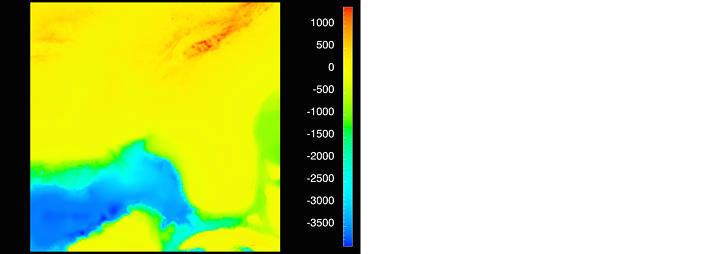
\includegraphics[scale=7.0]{florida_masked.jpg}
  \end{figure}
\end{frame}

\begin{frame}{Hating on the jet colour map}
  Did anybody see Florida?
  \begin{figure}[htp]
    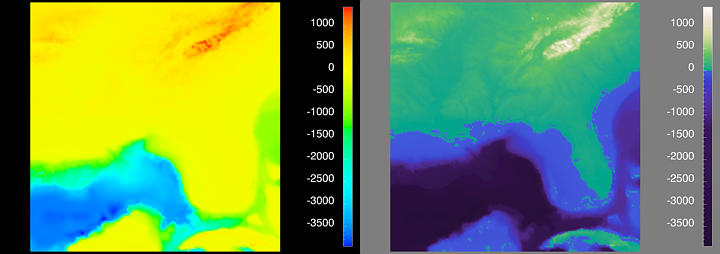
\includegraphics[scale=7.0]{florida.jpg}
  \end{figure}
\end{frame}

\begin{frame}
  \begin{center}
    Thank you.
  \end{center}
\end{frame}

\end{document}
